%\clearpage
\section{Risultati}
\label{sec:risultati}
Il programma sviluppato ha permesso di produrre numerosi risultati utili con quali sono state create le seguenti tracce per \acronimo{igv}:
\begin{description}
\item[\textsc{Unique sequence coverage}]: rappresenta la \emph{sequence coverage} delle \emph{unique read} trovate; i valori sono compresi tra $1$ e $80$;
\item[\textsc{Single sequence coverage}]: rappresenta la \emph{sequence coverage} delle \emph{single read} trovate; i valori sono compresi tra $1$ e $38$;
\item[\textsc{Multiple sequence coverage}]: rappresenta la \emph{sequence coverage} delle \emph{multiple read} trovate; i valori sono compresi tra $1$ e $118$;
\item[\textsc{Unique physical coverage}]: rappresenta la \emph{physical coverage} delle \emph{unique read} trovate; i valori sono compresa tra $1$ e $1386$;
\item[\textsc{Average insert length}]: rappresenta la lunghezza media degli inserti che iniziano in una certa posizione; la lunghezza media è uguale $2617 bp$ con una deviazione standard di $483 bp$;
\item[\textsc{Average discarded insert length}]: rappresenta la lunghezza media degli inserti che sono stati scartati in quanto fuori range; la soglia massima è stata scelta sfruttando i dati sulla lunghezza dei singoli inserti comparata con la loro media: è stato scelto un valore di $20000 bp$ in quanto ritenuto sufficientemente alto da non influire sui risultati.
\end{description}

\begin{figure}[htbp]
\centering
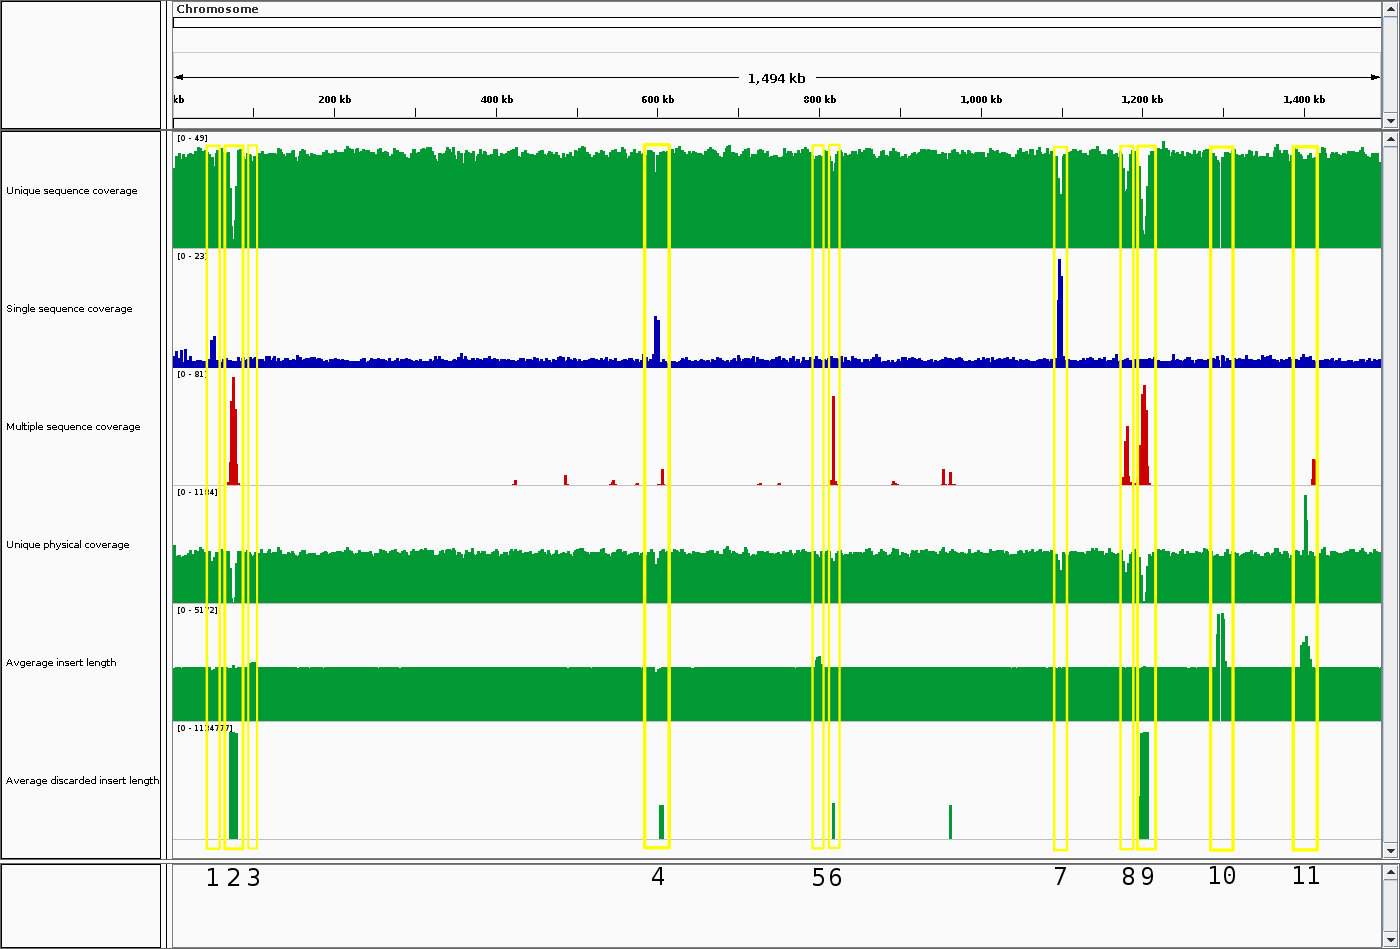
\includegraphics[width=\textwidth]{immagini/igv_global.png}
\caption{Vista globale delle tracce su IGV}
\label{fig:igv globale}
\end{figure}

La figura \ref{fig:igv globale} rappresenta le tracce appena descritte, i colori sono stati utilizzati per differenziare le tre tipologie di read a cui appartengono:
\begin{description}
\item[\textsc{Verde}]: identifica le tracce associate alle \emph{unique read};
\item[\textsc{Blu}]: identifica le tracce associate alle \emph{single read};
\item[\textsc{Rosso}]: identifica le tracce associate alle \emph{multiple read}.
\end{description}

Dai grafici si può notare come siano presenti diverse regioni interessanti all'interno delle tracce: sono quelle dove si vedono dei picchi in alcune di esse e avvallamenti nelle altre.

Le aree che a mio parere sono quelle più interessanti da valutare sono riquadrate con un rettangolo di colore giallo e per meglio identificarle sono numerate in ordine crescente.
Nel seguito verranno analizzate tali zone ed evidenziati i loro aspetti peculiari dando delle considerazioni sul possibile significato di variazione dei valori medi.
Le aree sono state raggruppate nel caso presentino aspetti comuni o pattern simili.

\subsection{Analisi regioni di interesse 1 e 4}
\begin{figure}[htbp]
	\centering
	\begin{subfigure}[b]{.45\textwidth}
		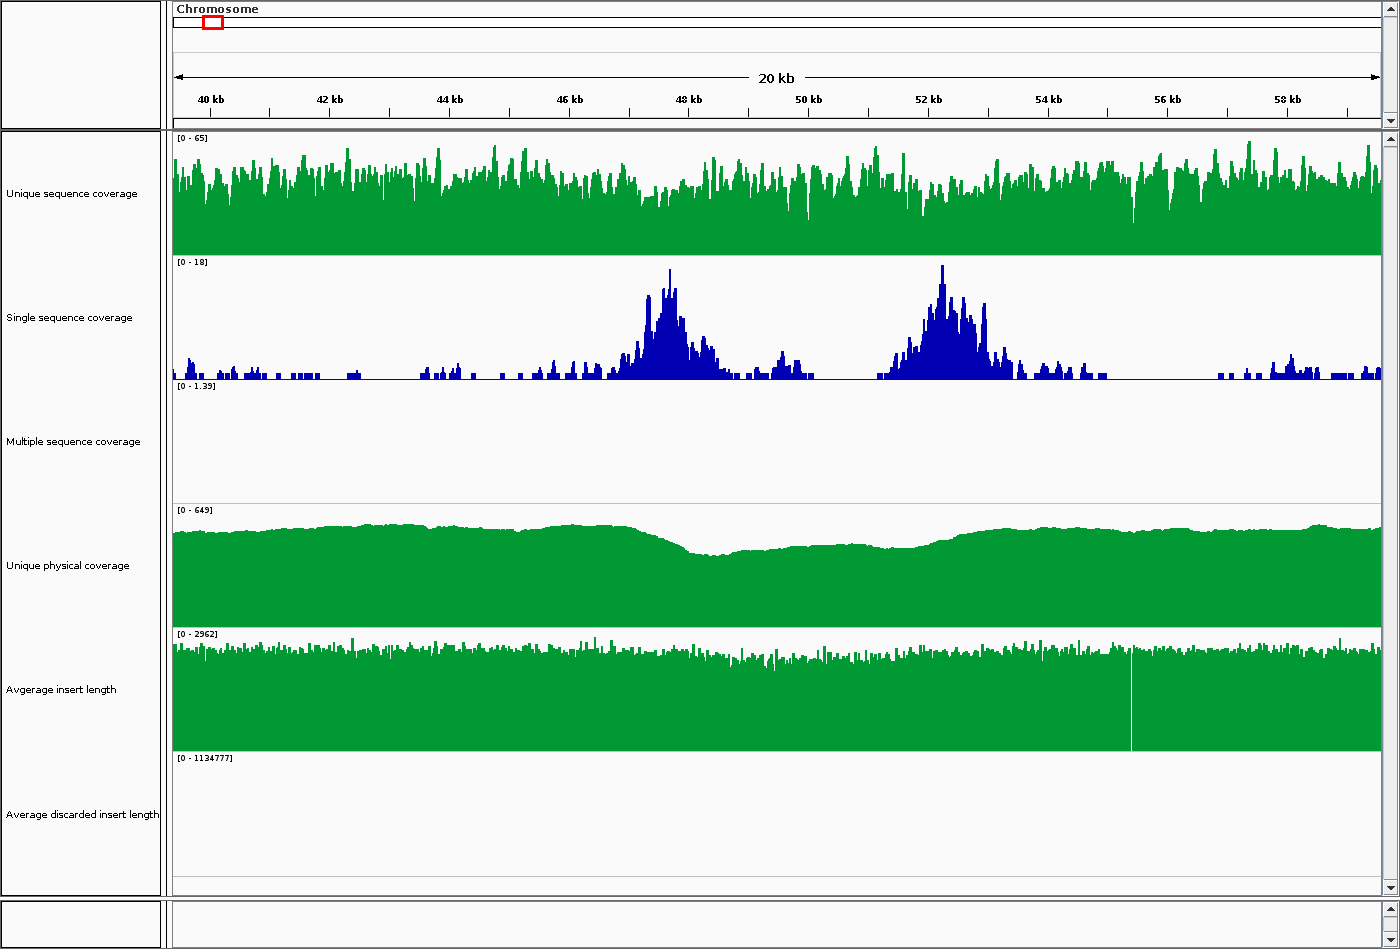
\includegraphics[width=\textwidth]{immagini/igv_regione1.png}
		\caption{Regione 1}
	\end{subfigure}
	\quad
	\begin{subfigure}[b]{.45\textwidth}
		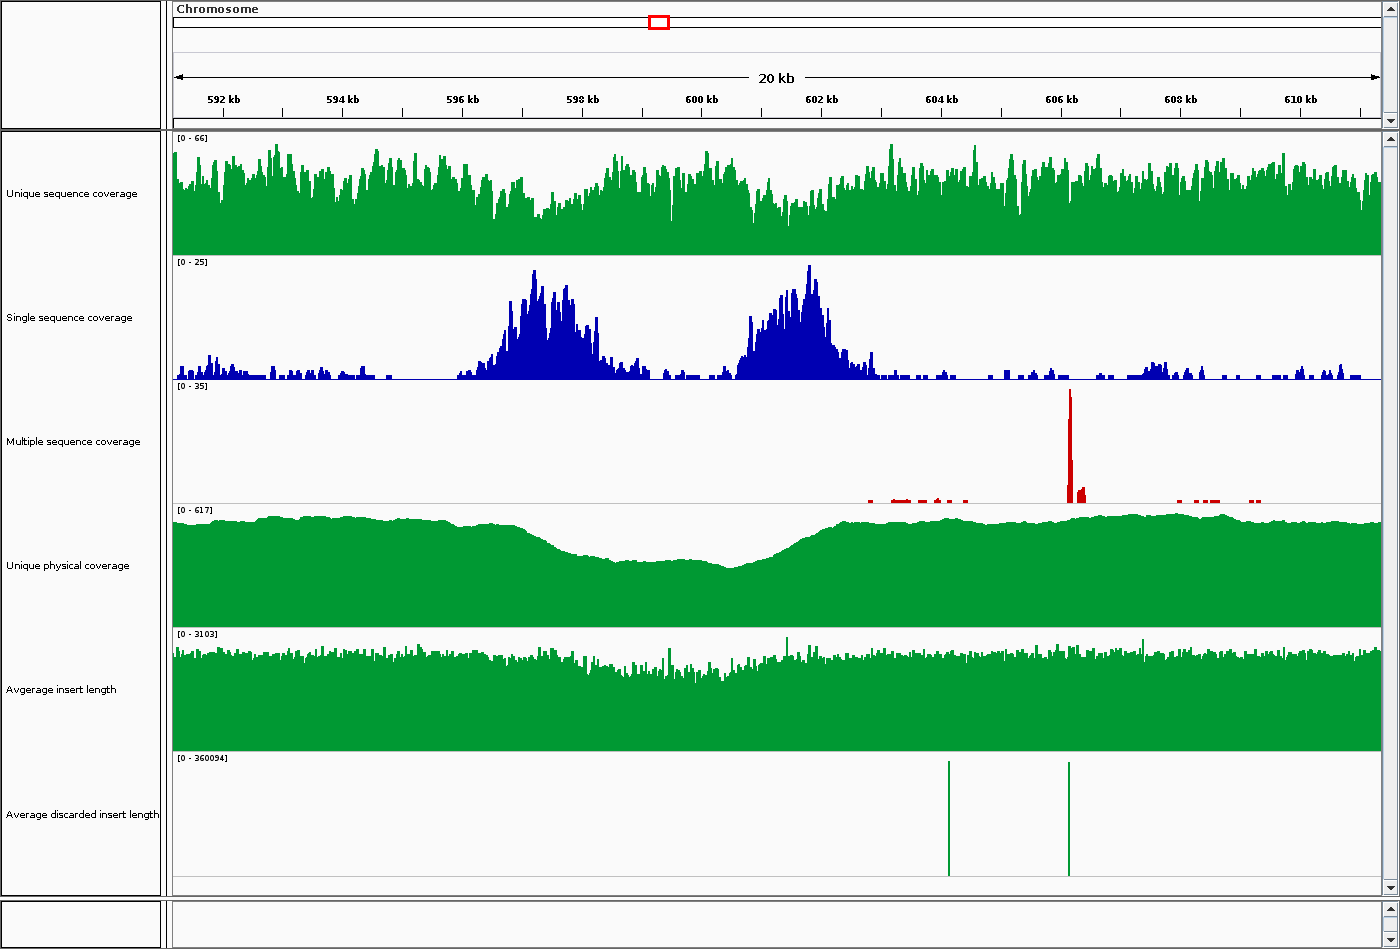
\includegraphics[width=\textwidth]{immagini/igv_regione4.png}
		\caption{Regione 4}
	\end{subfigure}
\caption{Regioni di interesse 1 e 4 su IGV}
\label{fig:regioni 1 e 4}
\end{figure}

In figura \ref{fig:regioni 1 e 4} si può notare come entrambe le regioni presentino due picchi nella \emph{sequence coverage} delle \emph{single read} mentre è presente una leggera diminuzione nella \emph{physical coverage} e in corrispondenza dei picchi la \emph{sequence coverage} delle \emph{unique read} presenta una leggera flessione: tale struttura potrebbe essere indicativa di brevi inserzioni dovute proprio alla presenza delle \emph{single read} e alla flessione della \emph{coverage}.

\subsection{Analisi regioni di interesse 2 e 9}
\begin{figure}[htbp]
	\centering
	\begin{subfigure}[b]{.45\textwidth}
		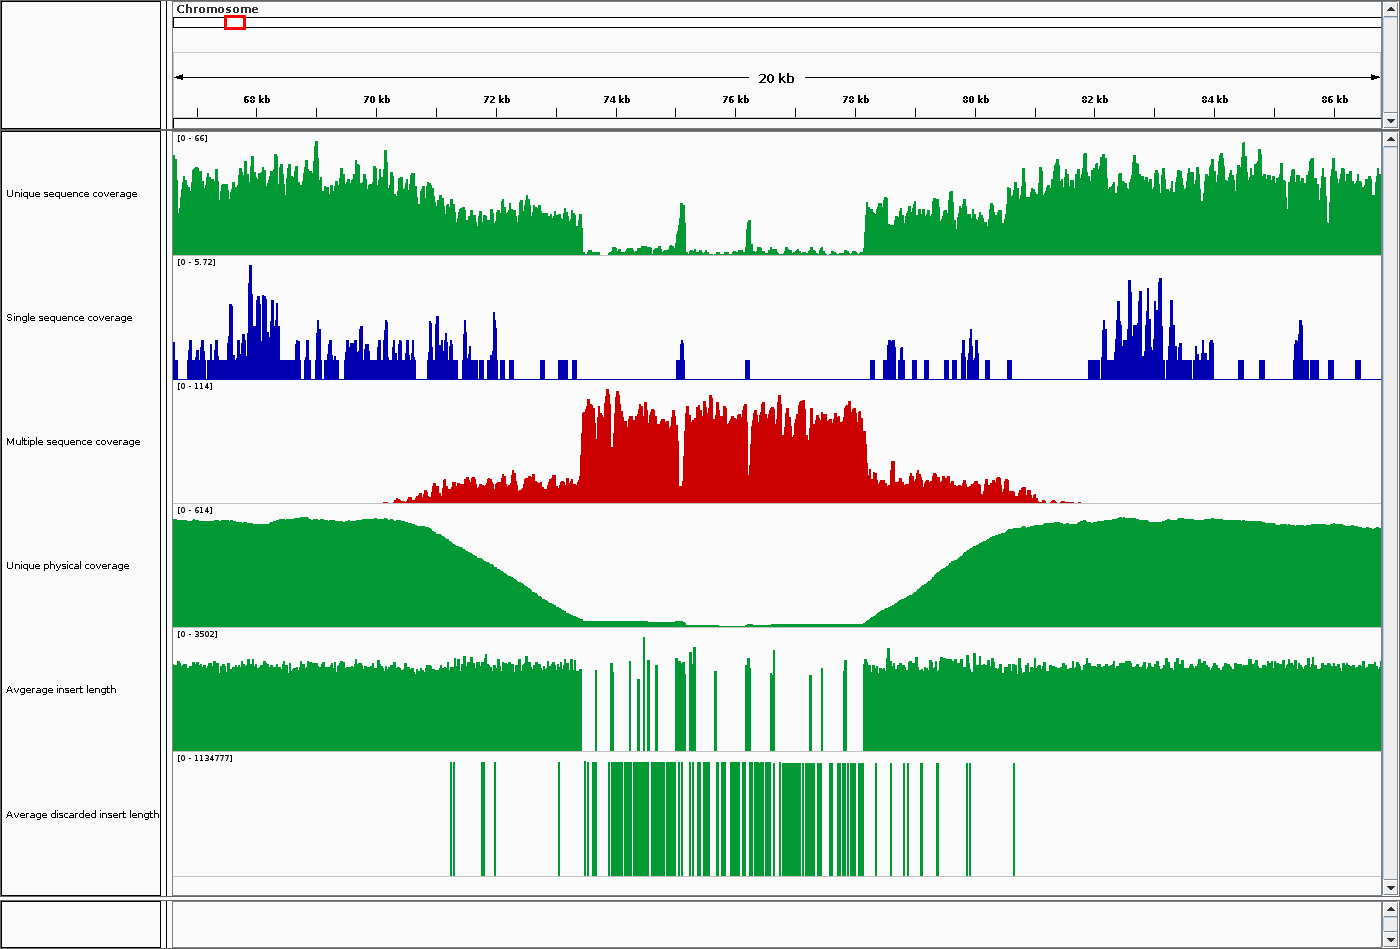
\includegraphics[width=\textwidth]{immagini/igv_regione2.png}
		\caption{Regione 2}
	\end{subfigure}
	\quad
	\begin{subfigure}[b]{.45\textwidth}
		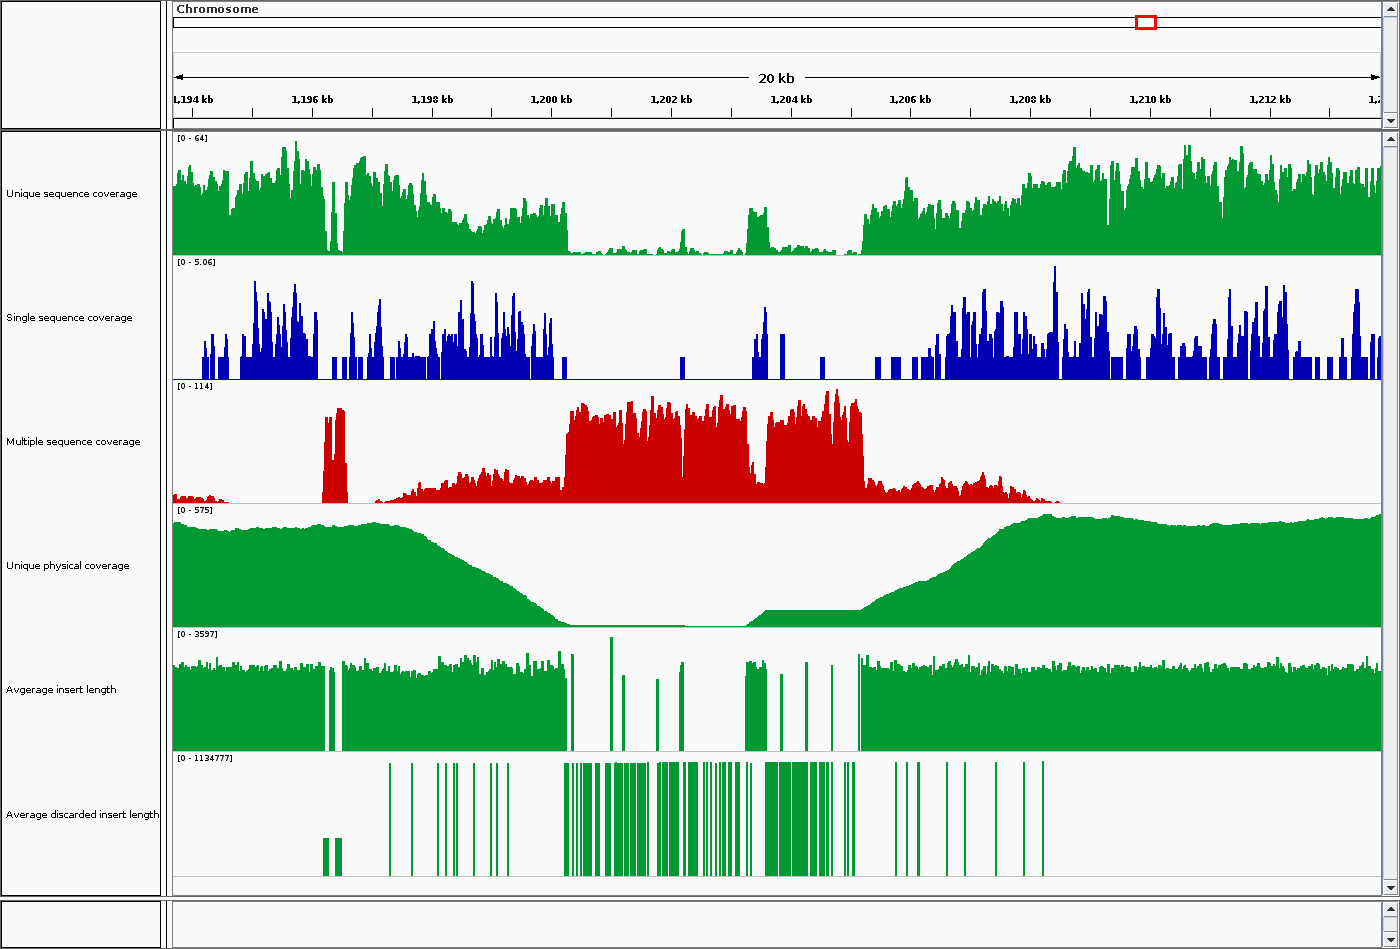
\includegraphics[width=\textwidth]{immagini/igv_regione9.png}
		\caption{Regione 9}
	\end{subfigure}
\caption{Regioni di interesse 2 e 9 su IGV}
\label{fig:regioni 2 e 9}
\end{figure}

Le immagini in figura \ref{fig:regioni 2 e 9} denotano la presenza di una notevole quantità di \emph{multiple read} che si sovrappone alla drastica diminuzione sia della \emph{physical} che della \emph{sequence coverage}.
Inoltre si può vedere come la lunghezza media degli inserti sia molto elevata.

Questi dati sono difficili da interpretare in quanto vi sarebbe la necessità di approfondire lo studio delle \emph{multiple read} per capire meglio le loro caratteristiche e individuare ulteriori \emph{mate pair}, se presenti.

\subsection{Analisi regioni di interesse 6 e 8}
\begin{figure}[htbp]
	\centering
	\begin{subfigure}[b]{.45\textwidth}
		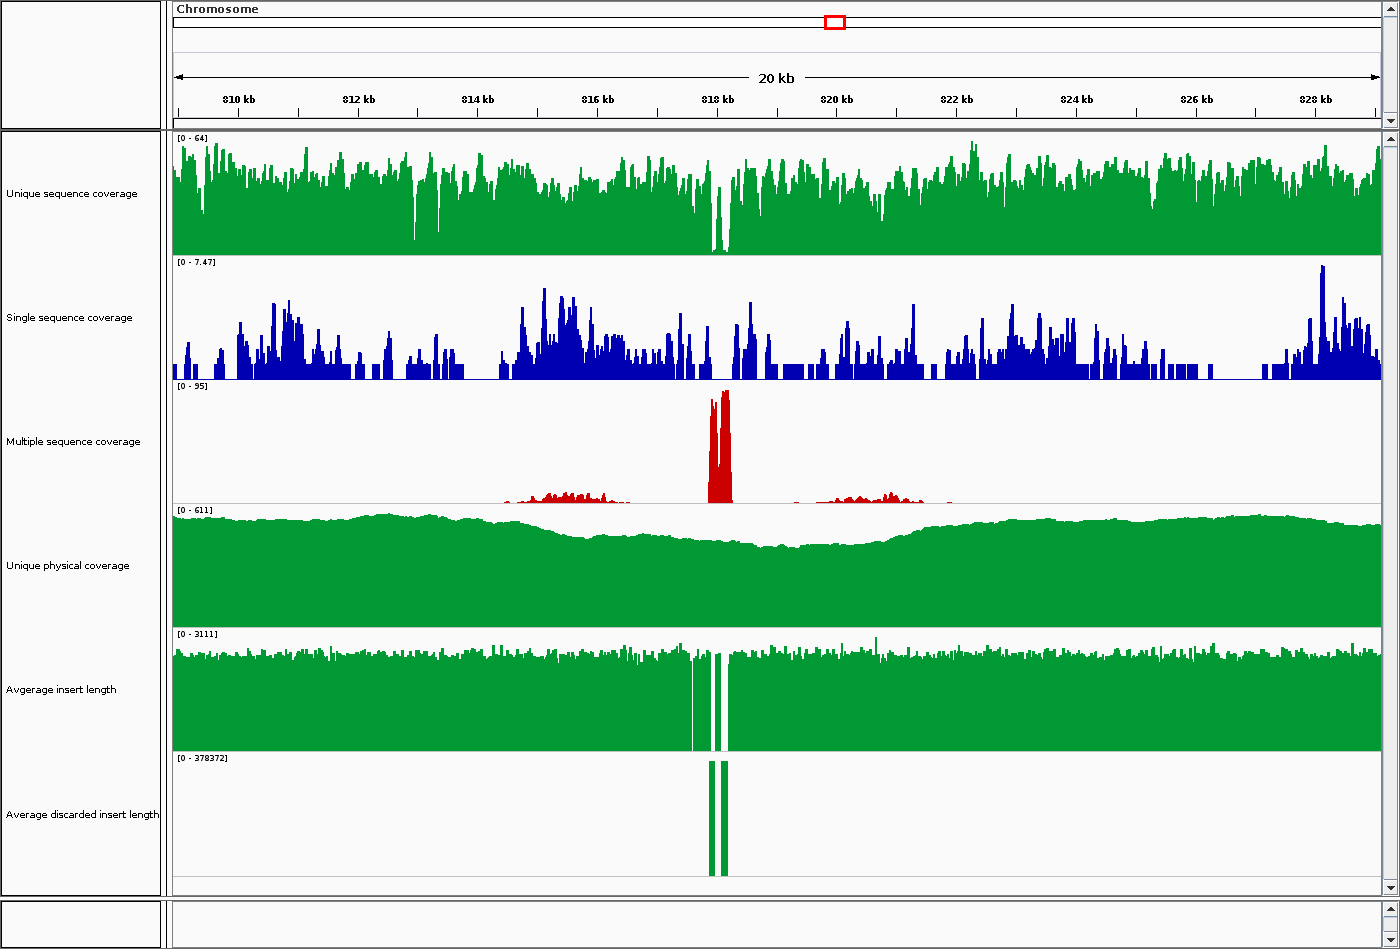
\includegraphics[width=\textwidth]{immagini/igv_regione6.png}
		\caption{Regione 6}
	\end{subfigure}
	\quad
	\begin{subfigure}[b]{.45\textwidth}
		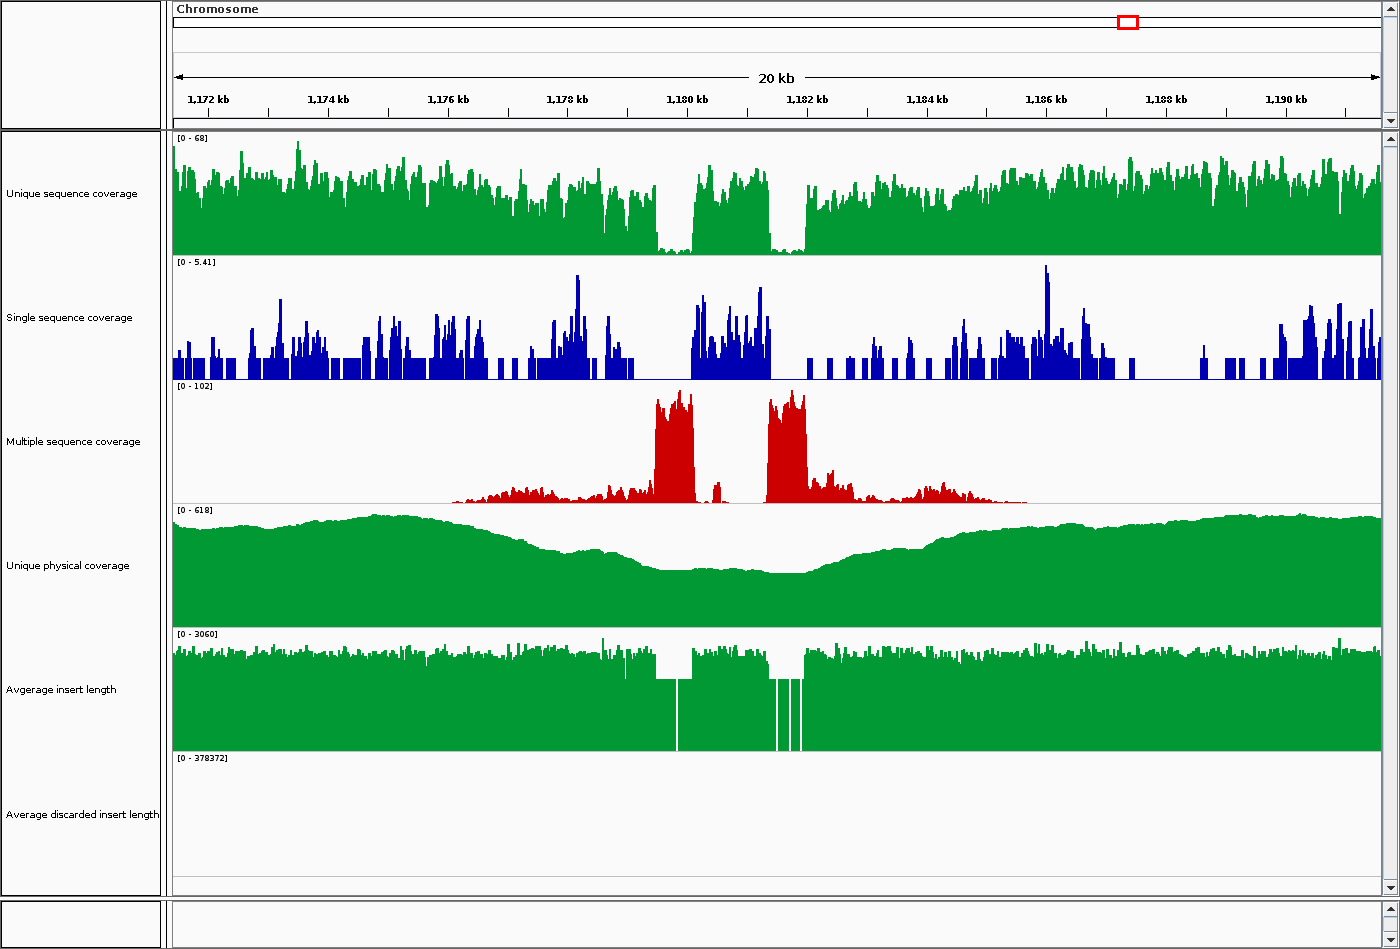
\includegraphics[width=\textwidth]{immagini/igv_regione8.png}
		\caption{Regione 8}
	\end{subfigure}
\caption{Regioni di interesse 6 e 8 su IGV}
\label{fig:regioni 6 e 8}
\end{figure}

Le regioni in figura \ref{fig:regioni 6 e 8} presentano caratteristiche simili a quelle in \ref{fig:regioni 2 e 9} ma si distinguono in quanto presentano due brevi picchi di \emph{multiple read} distinti che comportano una diminuzione nella \emph{sequence coverage} delle \emph{unique read} e nella \emph{physical coverage}.

Anche in questo caso l'unico modo di capire meglio la situazione è quello di indagare più approfonditamente le \emph{multiple read}.

\subsection{Analisi regioni di interesse 3, 5 e 10}
\begin{figure}[htbp]
	\centering
	\begin{subfigure}[b]{.45\textwidth}
		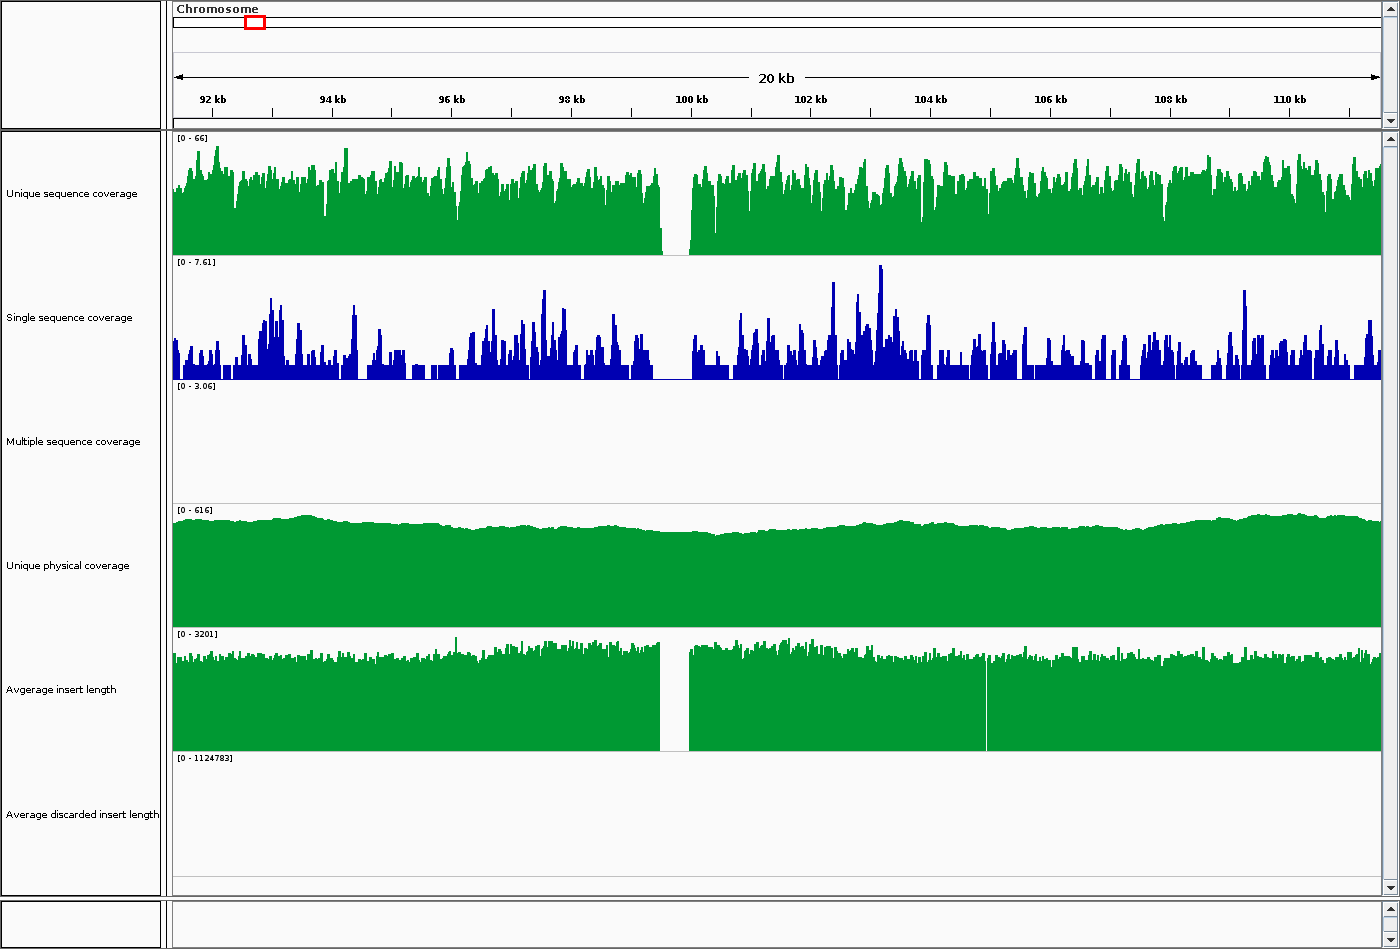
\includegraphics[width=\textwidth]{immagini/igv_regione3.png}
		\caption{Regione 3}
	\end{subfigure}
	\quad
	\begin{subfigure}[b]{.45\textwidth}
		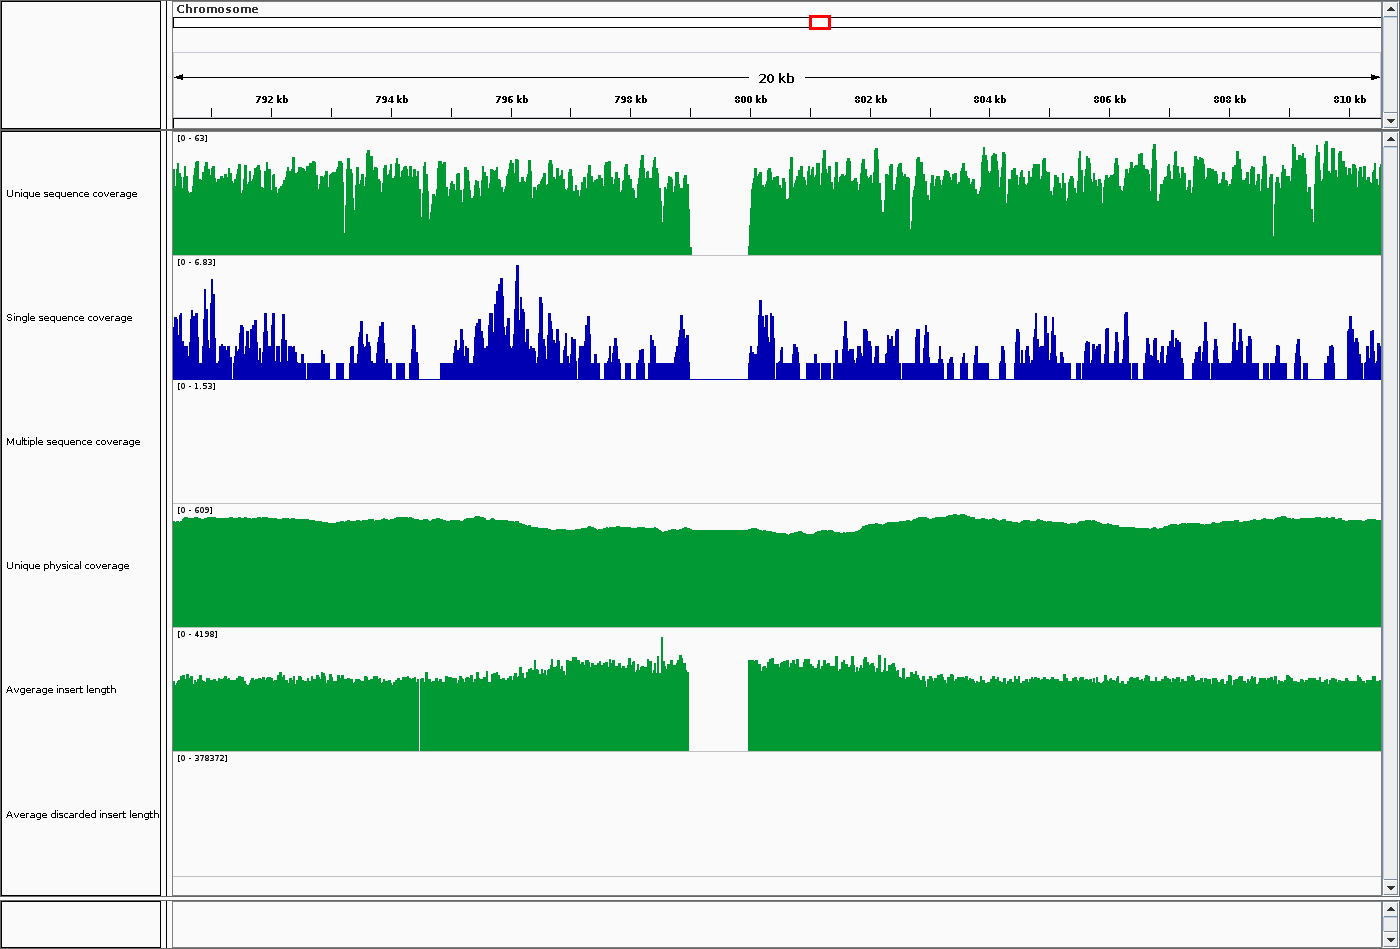
\includegraphics[width=\textwidth]{immagini/igv_regione5.png}
		\caption{Regione 5}
	\end{subfigure}
	\\[1em]
	\begin{subfigure}[b]{.45\textwidth}
		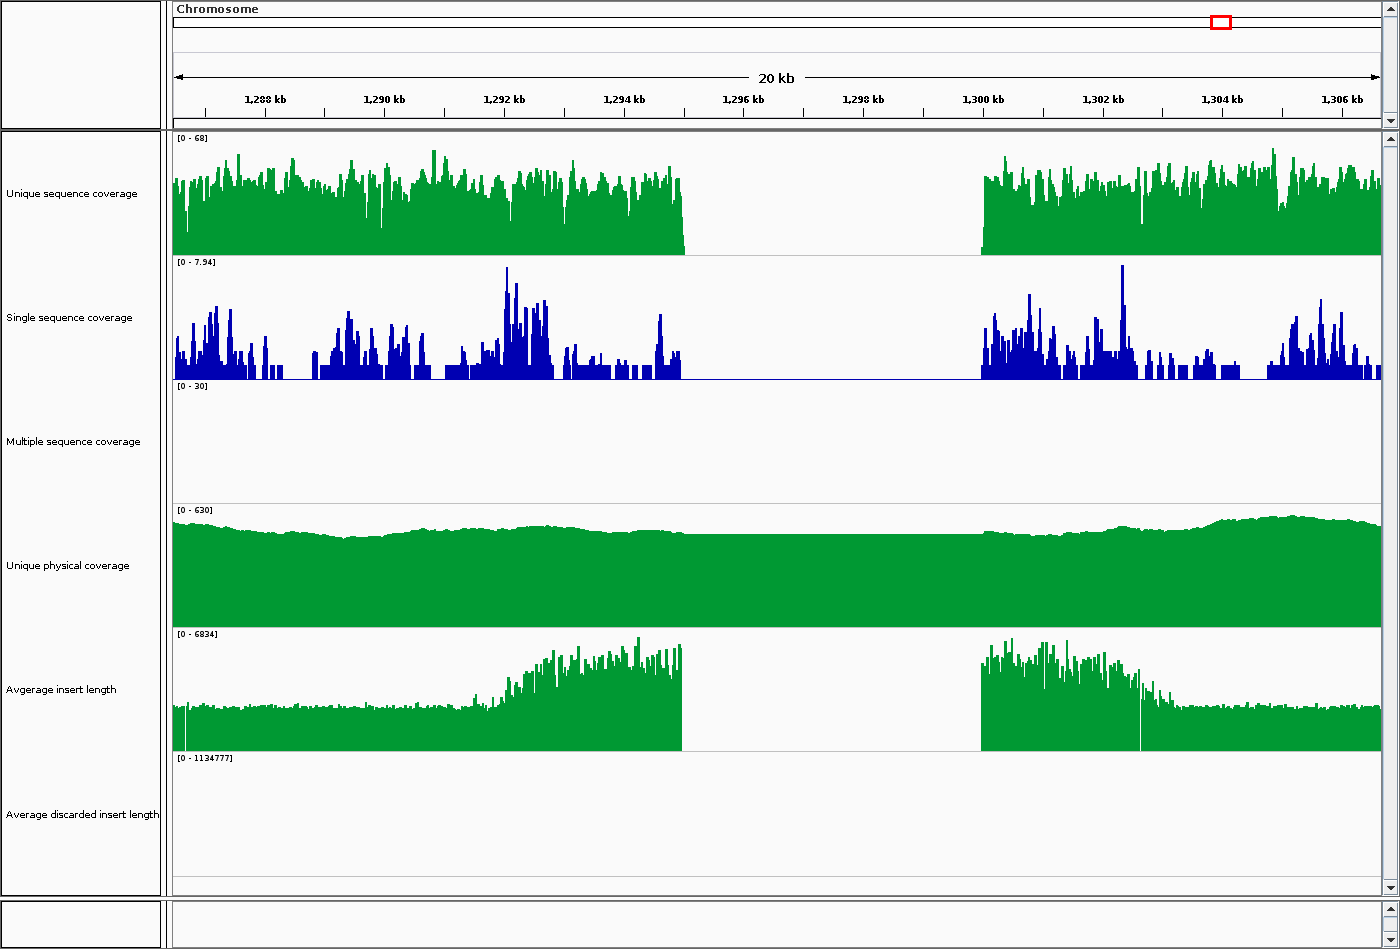
\includegraphics[width=\textwidth]{immagini/igv_regione10.png}
		\caption{Regione 10}
	\end{subfigure}
\caption{Regioni di interesse 3, 5 e 10 su IGV}
\label{fig:regioni 3, 5 e 10}
\end{figure}

In figura \ref{fig:regioni 3, 5 e 10} troviamo dei casi molto simili: tutti e tre presentano zone in cui non sono presenti read e questo indica sicuramente delle cancellazioni nel genoma.
L'unica differenza degna di nota è l'ampiezza di tali cancellazioni, sulle regioni $3$ e $5$ si aggira tra le $500bp$ e le $1000bp$ mentre nella regione 10 è nettamente superiore misurando circa $5kbp$.

\subsection{Analisi regione di interesse 7}
\begin{figure}[htbp]
	\centering
	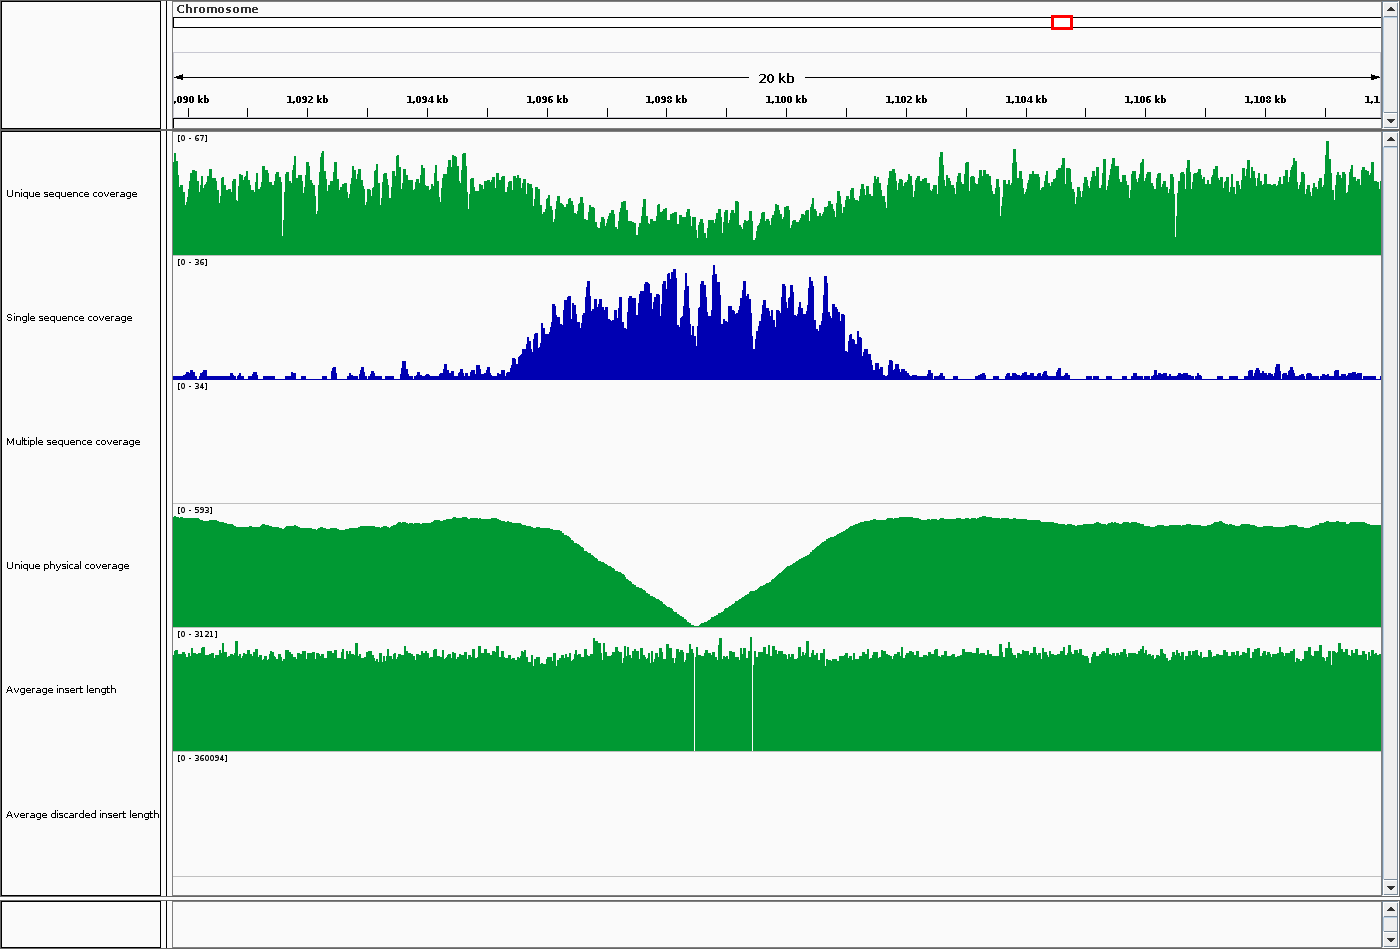
\includegraphics[width=.45\textwidth]{immagini/igv_regione7.png}
	\caption{Regione di interesse 7 su IGV}
	\label{fig:regione 7}
\end{figure}

La situazione rappresentata in figura \ref{fig:regione 7} è una chiara evidenza di una lunga inserzione in quanto si vede la \emph{physical coverage} creare il tipico aspetto a \emph{V} e la \emph{sequence coverage} delle \emph{unique read} scendere molto e quella delle \emph{single read} essere molto alta.

\subsection{Analisi regione di interesse 11}
\begin{figure}[htbp]
	\centering
	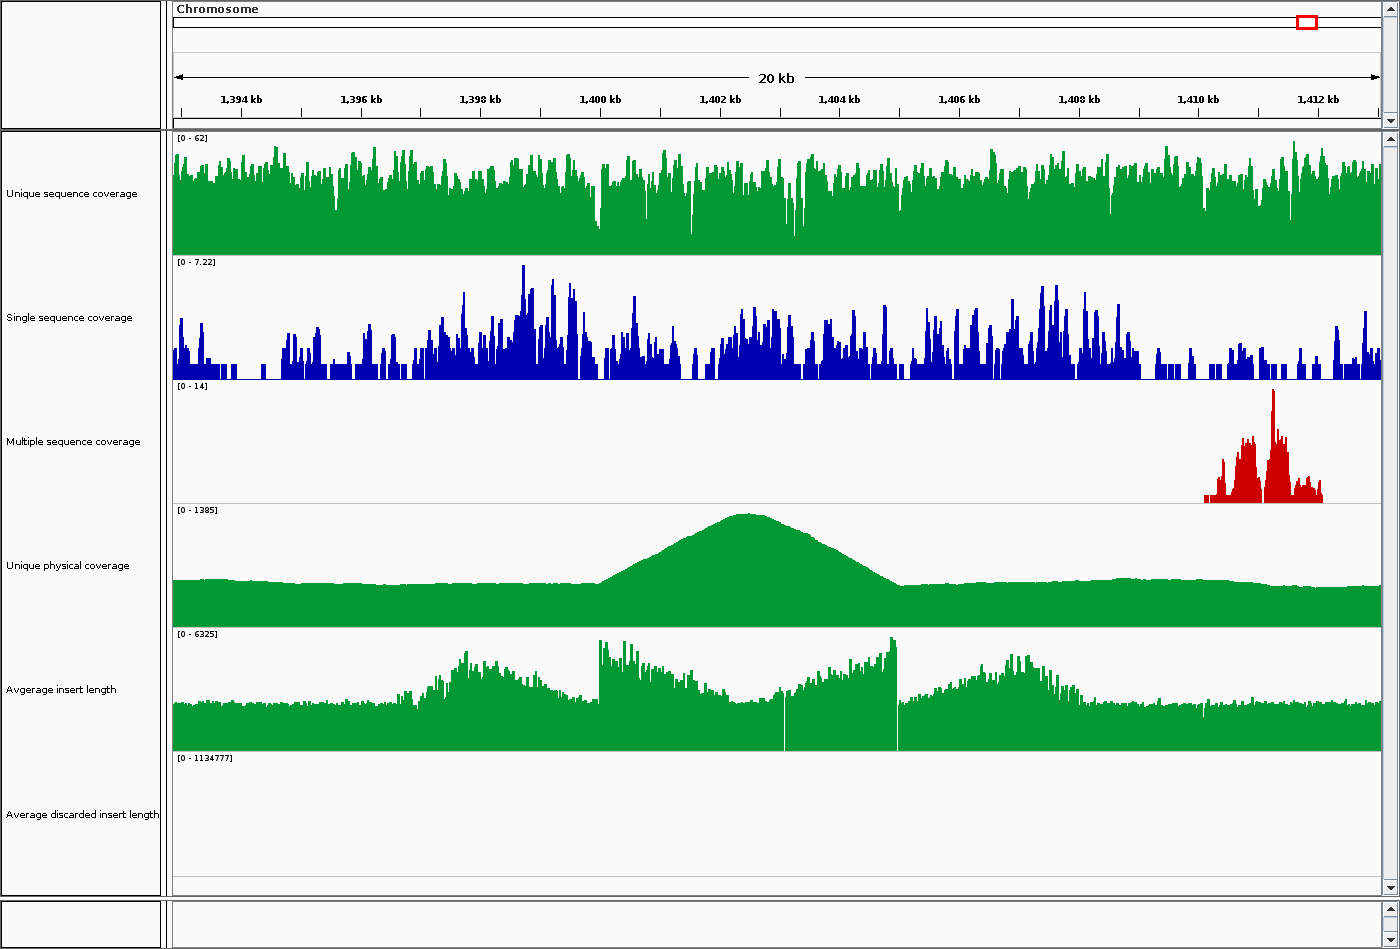
\includegraphics[width=.45\textwidth]{immagini/igv_regione11.png}
	\caption{Regione di interesse 11 su IGV}
	\label{fig:regioni 11}
\end{figure}

L'immagine in figura \ref{fig:regioni 11} presenta invece un aspetto per me insolito in quanto si evidenzia una forma a \emph{V} rovesciata in concomitanza di aumenti sensibili e simmetrici della lunghezza media degli inserti.

Per approfondire lo studio di questa area potrebbe essere interessante capire l'orientamento degli inserti per comprendere se può essere presente un'inversione.

\subsection{Analisi \emph{multiple read}}
Per quanto riguarda le \emph{multiple read} ho cercato un modo per effettuare un'analisi su di esse ma è risultata essere poco preciso in quanto è presente una notevole variabilità di caratteristiche tra le read.

Osservando a campione le read presenti nei file \acronimo{sam}, ho notato che tra i gruppi di tre e quattro read ci sono \emph{mate pair} che sono compatibili ma non sono riuscito a trovare dei criteri per sviluppare un algoritmo che riusca a discriminare bene ogni caso.

In particolare ho notato che in molti casi nei gruppi di tre read, due sono ad una distanza coerente con la media delle \emph{unique read}, mentre la terza è ad una distanza comparabile con quella degli inserti scartati perchè fuori range, questo si nota bene nelle figure \ref{fig:regioni 2 e 9} e \ref{fig:regioni 6 e 8}.

Invece nei gruppi di quattro read si potrebbero trovare due coppie di \emph{mate pair} con distanza compatibile anche se poste in due zone diverse del genoma a distanza molto elevata tra loro.

\subsection{Analisi \emph{unique read}}
Per lo studio delle \emph{unique read} ho effettuato un'analisi sulla loro lunghezza e ho prodotto una serie di grafici che sono serviti inizialmente a stimare un limite superiore per tali lunghezze: come descritto all'inizio della sezione \ref{sec:risultati} la media si attesta a $2617bp$ e di conseguenza ho deciso di utilizzare il valore di $20000bp$ per selezionare gli inserti.

\begin{figure}[htbp]
\centering
	\begin{subfigure}[b]{.45\textwidth}
	\includegraphics[width=\textwidth]{immagini/insert_length1.pdf}
	\caption{Grafico 1}
	\label{fig:grafico 1}
	\end{subfigure}
	\quad
	\begin{subfigure}[b]{.45\textwidth}
		\includegraphics[width=\textwidth]{immagini/insert_length1-1.pdf}
		\caption{Grafico 2}
		\label{fig:grafico 2}
	\end{subfigure}
	%\caption{Grafici relativi alla lunghezza degli inserti}
\end{figure}

In figura \ref{fig:grafico 1} si vede come siano presenti due aree dove le lunghezze degli inserti sono rispettivamente più corte e più lunghe della media.

\begin{figure}[htbp]
	\ContinuedFloat
	\centering
	\begin{subfigure}[b]{.45\textwidth}
		\includegraphics[width=\textwidth]{immagini/insert_length2.pdf}
		\caption{Grafico 3}
		\label{fig:grafico 3}
	\end{subfigure}
	%\caption{Grafici relativi alla lunghezza degli inserti}
\end{figure}
\begin{figure}[htbp]
	\ContinuedFloat
	\centering
	\begin{subfigure}[b]{.45\textwidth}
		\includegraphics[width=\textwidth]{immagini/insert_length3.pdf}
		\caption{Grafico 4}
		\label{fig:grafico 4}
	\end{subfigure}
	\quad
	\begin{subfigure}[b]{.45\textwidth}
		\includegraphics[width=\textwidth]{immagini/insert_length3-1.pdf}
		\caption{Grafico 5}
		\label{fig:grafico 5}
	\end{subfigure}
	%\caption{Grafici relativi alla lunghezza degli inserti}
\end{figure}

Anche in figura \ref{fig:grafico 5} il grafico presenta un area dove la lunghezza è minore rispetto alla media calcolata.

\begin{figure}[htbp]
	\ContinuedFloat
	\centering
	\begin{subfigure}[b]{.45\textwidth}	
		\includegraphics[width=\textwidth]{immagini/insert_length4.pdf}
		\caption{Grafico 6}
		\label{fig:grafico 6}
	\end{subfigure}
	\quad
	\begin{subfigure}[b]{.45\textwidth}
		\includegraphics[width=\textwidth]{immagini/insert_length4-1.pdf}
		\caption{Grafico 7}
		\label{fig:grafico 7}
	\end{subfigure}
	%\caption{Grafici relativi alla lunghezza degli inserti}
\end{figure}

In figura \ref{fig:grafico 6} invece si nota un aumento della lunghezza degli inserti.

\begin{figure}[htbp]
	\ContinuedFloat
	\centering
	\begin{subfigure}[b]{.45\textwidth}
		\includegraphics[width=\textwidth]{immagini/insert_length5.pdf}
		\caption{Grafico 8}
		\label{fig:grafico 8}
	\end{subfigure}
	%\caption{Grafici relativi alla lunghezza degli inserti}
\end{figure}
\begin{figure}[htbp]
	\ContinuedFloat
	\centering
	\begin{subfigure}[b]{.45\textwidth}
		\includegraphics[width=\textwidth]{immagini/insert_length6.pdf}
		\caption{Grafico 9}
		\label{fig:grafico 9}
	\end{subfigure}
	\quad
	\begin{subfigure}[b]{.45\textwidth}
		\includegraphics[width=\textwidth]{immagini/insert_length6-1.pdf}
		\caption{Grafico 10}
		\label{fig:grafico 10}
	\end{subfigure}
	%\caption{Grafici relativi alla lunghezza degli inserti}
\end{figure}

I grafici nelle figure \ref{fig:grafico 9} e \ref{fig:grafico 10} presentano anch'esse un aumento della lunghezza di alcuni inserti ma in questo caso la variazione è superiore che nei casi esaminati in precedenza.

\begin{figure}[htbp]
	\ContinuedFloat
	\centering
	\begin{subfigure}[b]{.45\textwidth}
		\includegraphics[width=\textwidth]{immagini/insert_length7.pdf}
		\caption{Grafico 11}
		\label{fig:grafico 11}
	\end{subfigure}
	\caption{Grafici relativi alla lunghezza degli inserti}
\end{figure}
\begin{figure}[htbp]
	\centering
	\includegraphics[width=.45\textwidth]{immagini/discarded_insert_length.pdf}
	\caption{Grafici relativi alla lunghezza degli inserti scartati}
	\label{fig:discarded insert length}
\end{figure}

L'ultimo grafico in figura \ref{fig:discarded insert length} evidenzia gli inserti con una lunghezza incompatibile che si attesta intorno alle $1100kbp$: sono stati trovati solamente $199$ inserti fuori range e sono quindi un numero davvero ristretto.

Le variazioni nella lunghezza trovate nelle \emph{unique read} sono riscontrabili anche negli screenshot tratti da \acronimo{igv}: le diminuzioni e gli aumenti sono riconducibili rispettivamente a dei cali e degli incrementi nella \emph{physical coverage}.